\chapter{Sets and Maps}
During the first term we have seen how useful \blue{sets} and \blue{dictionaries} are.  The abstract concept
that is implemented as a dictionary in \textsl{Python} is known as a \blue{map} in theoretical computer science.
The main idea behind a map is to have a function that is defined on a finite set of \blue{keys} that
maps these keys to \blue{values}.  A typical example of a map is a telephone book.  In that case, the keys
are names, while the values are the telephone numbers associated with these names.

In this chapter we will see how sets and maps can be implemented efficiently.  We confine our attention to the
implementation of maps.  Once we know how to implement a map, it is easy to see that a set $S$ can be
represented by a function $f_S$ that satisfies 
\\[0.2cm]
\hspace*{1.3cm}
$x \in S \Leftrightarrow f_S(x) \not= \Omega$.
\\[0.2cm]
The rest of this chapter is organized as follows:
\begin{enumerate}[(a)]
\item We begin with the definition of the abstract data type \blue{Map}. 
    
      Following this definition we present several different implementations of maps. 
\item We start our discussion with \blue{ordered binary trees}.  These trees can be used to implement maps,
      provided the keys are ordered.  The average complexity of finding the value associated with a key
      is $\Oh\bigl(\log_2(n)\bigr)$, where $n$ is the number of key-value pairs stored in the binary tree.
      Unfortunately, the worst case complexity  is $\Oh(n)$.
\item Next, we discuss \blue{balanced ordered trees}.  In the case of balanced ordered trees the
      complexity of finding the value associated with a given key is g\underline{uaranteed} to be
      \blue{logarithmic} in the number of keys, i.e.~it is $\Oh\bigl(\log_2(n)\bigr)$.
      There are many different kinds of balanced ordered trees.  In this lecture notes we will discuss
      \blue{AVL trees} and \blue{2-3 trees}. 
\item After that, we explore a data structure that is known as a \blue{trie}.  This kind of data structure can
      be used if the keys of the map are \blue{strings}. 
\item Finally, we discuss \blue{hash tables}.  Hash tables provide another way to implement a map.
      Hash tables are in wide spread use.  For example, in \textsl{Python} sets and dictionaries are
      implemented via hash tables.  Therefore, every computer scientist should have a good understanding of
      their inner workings. 
\end{enumerate}

\section{The Abstract Data Type Map} 
Many applications require the efficient maintenance of some mapping of \blue{keys} to
\blue{values}.  For example, in order to implement a software analogue of a telephone book we have to
be able to associate the name of a person with their telephone number.  In this case, the name of a person is
regarded as a \blue{key} and the telephone number is the \blue{value} that gets associated with the key.
The most important functions provided by a telephone directory are the following:
\begin{enumerate}
\item \blue{Lookup}: We have to be able to look up a given name and return the telephone number
      associated with this name.
\item \blue{Insertion}: We need to be able to insert a new name and the corresponding telephone
      number into our directory.
\item \blue{Deletion}: The final requirement is that it has to be possible to delete names from
      the directory.
\end{enumerate}


\begin{Definition}[Map] \hspace*{\fill} \\
  The abstract data type of a \blue{Map} is defined as follows:
  \begin{enumerate}
  \item The name is \textsl{Map}.
  \item The set of type parameters is $\{ \textsl{Key}, \textsl{Value} \}$.
  \item The set of function symbols is \\[0.1cm]
       \hspace*{1.3cm} 
       $\{ \mytt{map}, \mytt{find}, \mytt{insert}, \mytt{delete} \}$.
  \item The signatures of these function symbols are as follows:
        \begin{enumerate}
        \item $\mytt{map}: \textsl{Map}$

              Calling $\mytt{map}()$ generates a new empty map.  Here, an empty map is a map that
              does not store any keys.
        \item $\mytt{find}: \textsl{Map} \times \textsl{Key} \rightarrow \textsl{Value} \cup \{\Omega\}$

              The function call
              \\[0.2cm]
              \hspace*{1.3cm}
              $m.\mytt{find}(k)$ 
              \\[0.2cm]
              checks whether the key $k$ is stored in the map $m$.  If this is the case, the
              value associated with this key is returned, otherwise the function call returns
              the undefined value $\Omega$.
        \item $\mytt{insert}: \textsl{Map} \times \textsl{Key} \times \textsl{Value} \rightarrow \textsl{Map}$

              The function call
              \\[0.2cm]
              \hspace*{1.3cm}
              $m.\mytt{insert}(k,v)$ 
              \\[0.2cm]
              takes a key $k$ and an associated value $v$ and stores this information into the map
              $m$.  If the map $m$ already stores a value associated with the key $k$, this value
              is overwritten.  

              The function call returns the resulting map.
        \item $\mytt{delete}: \textsl{Map} \times \textsl{Key} \rightarrow \textsl{Map}$

              The function call
              \\[0.2cm]
              \hspace*{1.3cm}
              $m.\mytt{delete}(k)$ 
              \\[0.2cm]
              removes the key $k$ and any value associated with $k$ from the map $m$.  If the map $m$ does not contain a value for the
              key $k$, then the map is returned unchanged.

              The function call returns the new map. 
        \end{enumerate}
  \item The behaviour of a map is specified via the following axioms.
        \begin{enumerate}
        \item $\mytt{map}().\mytt{find}(k) = \Omega$.

              Calling $\mytt{map}()$ generates an empty map which does not have any keys stored.
              Hence, looking up any key in the empty map will just return the undefined value.
        \item $m.\mytt{insert}(k, v).\mytt{find}(k) = v$.

              If a value $v$ is inserted for a key $k$, then when we look up this key $k$ the corresponding value
              $v$ will be returned.
        \item $k_1 \not= k_2 \rightarrow m.\mytt{insert}(k_1, v).\mytt{find}(k_2) = m.\mytt{find}(k_2)$.

              If a value $v$ is inserted for a key $k_1$, then this does not change the value that is stored
              for any key $k_2$  different from $k_1$.
        \item $m.\mytt{delete}(k).\mytt{find}(k\bigr) = \Omega$.

              If the key $k$ is deleted, then afterwards we won't find this key anymore.
        \item $k_1 \not= k_2 \rightarrow 
               m.\mytt{delete}(k_1).\mytt{find}(k_2) = m.\mytt{find}(k_2)$,

              If  we delete a key $k_1$ and then try to look up the information stored under a key
              $k_2$ that is different from $k_1$, we will get the same result that we would have gotten
              if we had searched for $k_2$ before deleting $k_1$.
              \eox
        \end{enumerate}
  \end{enumerate}
\end{Definition}

In \textsl{Python} it is very easy to implement the abstract data type  \textsl{Map}.  We just have
to realize that a map is essentially the same thing as a dictionary.
Now if $d$ is a dictionary storing the value $v$ for a key $k$, then the expression
\\[0.2cm]
\hspace*{1.3cm} $d[k]$
\\[0.2cm]
returns the value $v$.  On the other hand we can insert a value $v$ for a key $k$ by
writing
\\[0.2cm]
\hspace*{1.3cm}
$d[k] = v$ 
\\[0.2cm]
and in order to delete the value stored for a key  $k$ we can use the \mytt{del} statement
as follows: \\[0.2cm]
\hspace*{1.3cm} $\mytt{del}\ d[k]$. \\[0.2cm]
Figure  \ref{fig:Map-Trivial.ipynb} presents an implementation of the class \mytt{Map} that proceeds along
these lines.


\begin{figure}[!ht]
  \centering
\begin{minted}[ frame         = lines, 
                framesep      = 0.3cm,
                bgcolor       = sepia,
                numbers       = left,
                numbersep     = -0.2cm,
                xleftmargin   = 0.8cm,
                xrightmargin  = 0.8cm
              ]{python3}
    class Map:
        def __init__(self):
            self.mDictionary = {}
        
        def find(self, k):
            return self.mDictionary[k]
        
        def insert(self, k, v):
            self.mDictionary[k] = v
            
        def delete(self, k):
            del self.mDictionary[k]
            
        def __str__(self):
            return str(self.mDictionary)
\end{minted}
\vspace*{-0.3cm}
  \caption{A trivial implementation of the abstract data type \textsl{Map} in \textsl{Python}.}
  \label{fig:Map-Trivial.ipynb}
\end{figure} 
Note that the methods \mytt{insert} and \mytt{delete} do not return an object of type \mytt{Map}.  Rather, for
efficiency reasons, the existing \mytt{Map} object is updated.


\section{Ordered Binary Trees}
If the set \textsl{Key} is linearly ordered, i.e.~if there exists a binary relation
$\leq \;\subseteq\textsl{Key}\times\textsl{Key}$ such that the pair $\langle \textsl{Key}, \leq \rangle$ is a linear
order, then the abstract data type \textsl{Map} can be implemented via  
\href{https://en.wikipedia.org/wiki/Binary_search_tree}{\blue{ordered binary trees}} also known as
\blue{binary search trees}. 
The implementation of the ADT map that is based on ordered binary trees has the following performance
characteristics: 
\begin{enumerate}
\item In the average case, the complexity of the method \mytt{find} is \blue{logarithmic} in the number of entries.
\item In the worst case, the complexity of the method \mytt{find} is \blue{linear} in the number of entries.

      Unfortunately, the worst case occurs when the keys are inserted in sorted order.
\end{enumerate}

\begin{Definition}[Ordered Binary Trees] \index{ordered binary tree} \hspace*{\fill} \\
  Assume a set $\textsl{Key}$ and a set $\textsl{Value}$ are given.
  The set $\Bin$ of \blue{ordered binary trees} \index{$\mathcal{B}$, set of ordered binary trees} is defined
  inductively as the set of \blue{terms} that are constructed from the function symbols \mytt{Nil} and
  \mytt{Node}, where the signatures of these function symbols are given as follows: \\[0.2cm]
  \hspace*{1.3cm} 
  $\mytt{Nil}\!:\; \Bin$ \qquad and \qquad  $\mytt{Node}\!:\; \textsl{Key} \times \textsl{Value} \times \Bin \times \Bin \rightarrow \Bin$.
  \begin{enumerate}
  \item $\mytt{Nil}$ is an ordered binary tree. \index{\mytt{Nil}, empty tree}

        This tree is called the \blue{empty tree} \index{empty tree} since it does not store any information.
  \item $\mytt{Node}(k, v, l, r) \in \Bin$ \quad iff the following conditions hold: \index{$\mytt{Node}(k, v, l, r)$}
        \begin{enumerate}
        \item $k$ is a key from the set $\textsl{Key}$.
        \item $v$ is a value from the set $\textsl{Value}$.
        \item $l$ is an ordered binary tree.

              $l$ is the  \blue{left subtree} \index{left subtree} of the tree $\mytt{Node}(k, v, l, r)$.
        \item $r$ is a ordered binary tree.

              $r$ is the \blue{right subtree} \index{right subtree} of the tree $\mytt{Node}(k, v, l, r)$.
        \item All keys that occur in the left subtree $l$ are smaller than $k$.
        \item All keys that occur in the right subtree $r$ are bigger than $k$.
        \end{enumerate}
        The last two conditions are known as the \blue{ordering conditions}. \index{ordering conditions}
        \eox
\end{enumerate}
\end{Definition}

\noindent
We will depict ordered binary trees graphically as follows:
\begin{enumerate}
\item The empty tree \mytt{Nil} is either shown as a black dot $\bullet$ or it is not shown at all.
\item A binary tree of the form $\mytt{Node}(k,v,l,r)$ is represented by an oval.  Inside of this
      oval, both the key $k$ and the value $v$ are printed.  The key is printed above the value and
      both are separated by a horizontal line.  This oval is then called a
      \blue{node} \index{node of a binary tree} of the binary tree. 
      The left subtree $l$ of the node is depicted to the south-west of the node,
      while the right subtree $r$ is depicted to the south-east of the node.  Both the left
      and the right subtree are connected to the node with an arrow that points from the node to the
      subtree.
\end{enumerate}
Figure \ref{fig:graph1} shows an example of an ordered binary tree.  The topmost node, that is the
node that has the key $8$ and the value $22$ is called the \blue{root} \index{root of a binary tree} of the binary tree.
A \blue{path of length} $k$ in the tree is a list $[n_0,n_1, \cdots, n_k]$ of
$k+1$ nodes that are connected via arrows.  If we identify nodes with their labels, we have that
\\[0.2cm]
\hspace*{1.3cm} $\bigl[ \pair(8,22), \pair(12,18), \pair(10,16), \pair(9,39) \bigr]$ \\[0.2cm]
is a path of length 3.


\begin{figure}[!ht]
  \centering
  \framebox{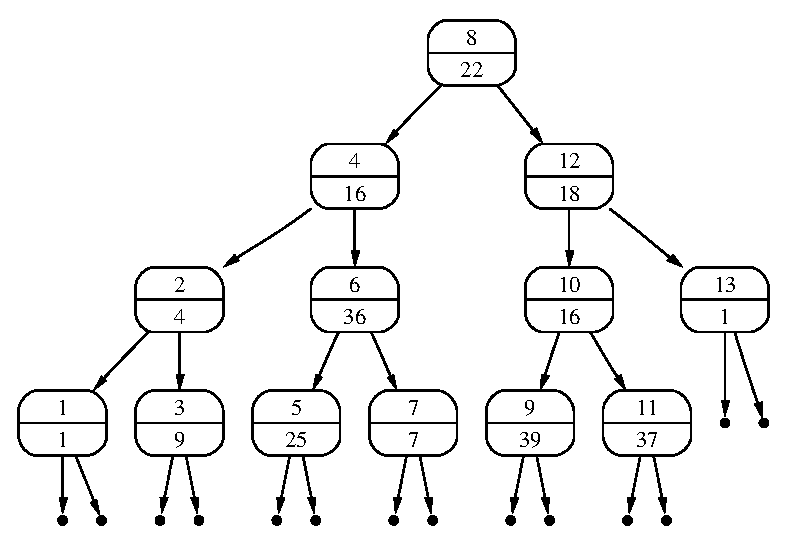
\epsfig{file=Abbildungen/graph1.eps}} 
  \caption{An ordered binary tree.}
  \label{fig:graph1}
\end{figure}


Next, we show how ordered binary trees can be used to implement the ADT  \textsl{Map}.  We specify
the different methods of this ADT via conditional equations.  The constructor $\mytt{map}()$
returns the empty tree:
\\[0.2cm]
\hspace*{1.3cm}
$\mytt{map}() = \mytt{Nil}$. 
\\[0.2cm]
The  method $\mytt{find}$ has the signature \index{\mytt{find}, ordered binary tree}
\\[0.2cm]
\hspace*{1.3cm}
$\mytt{find}:\mathcal{B} \times \textsl{Key} \rightarrow \textsl{Value} \cup \{ \Omega \}$
\\[0.2cm]
and is specified as follows:
\begin{enumerate}
\item $\mytt{Nil}.\mytt{find}(k) = \Omega$,

      because the empty tree is interpreted as the empty map.
\item $\mytt{Node}(k, v, l, r).\mytt{find}(k) = v$,

      because the node $\mytt{Node}(k,v,l,r)$ stores the assignment $k \mapsto v$.
\item $k_1 < k_2 \rightarrow \mytt{Node}(k_2, v, l, r).\mytt{find}(k_1) = l.\mytt{find}(k_1)$,

      because if $k_1$ is less than $k_2$, then any mapping for $k_1$ has to be stored in the left
      subtree  $l$.
\item $k_1 > k_2 \rightarrow \mytt{Node}(k_2, v, l, r).\mytt{find}(k_1) = r.\mytt{find}(k_1)$,

      because if $k_1$ is greater than $k_2$, then any mapping for $k_1$ has to be stored in the right
      subtree  $r$.
\end{enumerate}
Next, we specify the method  \mytt{insert}.  The signature of \mytt{insert} is
\\[0.2cm]
\hspace*{1.3cm}
$\mytt{insert}: \mathcal{B} \times \textsl{Key} \times \textsl{Value} \rightarrow \mathcal{B}$
\\[0.2cm]
and the definition of \mytt{insert} is given by the following equations.
\index{\mytt{insert}, ordered binary tree}
\begin{enumerate}
\item $\mytt{Nil}.\mytt{insert}(k,v) = \mytt{Node}(k,v, \mytt{Nil}, \mytt{Nil})$,
  
      If the tree is empty, the information to be stored is placed at the root.
\item $\mytt{Node}(k,v_2,l,r).\mytt{insert}(k,v_1) = \mytt{Node}(k, v_1, l, r)$,

      If the key $k$ is located at the root, we can just overwrite the old information. 
\item $k_1 < k_2 \rightarrow 
         \mytt{Node}(k_2, v_2, l, r).\mytt{insert}(k_1, v_1) = \mytt{Node}(k_2, v_2, l.\mytt{insert}(k_1, v_1), r)$,

      If the key $k_1$, which is the key for which we want to store a value, is less than the key
      $k_2$ at the root, then we have to insert the information in the left subtree.
\item $k_1 > k_2 \rightarrow 
         \mytt{Node}(k_2, v_2, l, r).\mytt{insert}(k_1, v_1) = 
         \mytt{Node}(k_2, v_2, l, r.\mytt{insert}(k_1, v_1))$,

      If the key $k_1$, which is the key for which we want to store a value, is bigger than the key
      $k_2$ at the root, then we have to insert the information in the right subtree.
\end{enumerate}
Finally we specify the method  \mytt{delete}.  The signature is
\\[0.2cm]
\hspace*{1.3cm}
$\mytt{delete}: \mathcal{B} \times \textsl{Key} \rightarrow \mathcal{B}$.
\\[0.2cm]
\index{\mytt{delete}, ordered binary tree}
The specification of \mytt{delete} is more difficult than the specification of \mytt{find} and
\mytt{insert}. If there is a tree of the form $t =\mytt{Node}(k,v,l,r)$ and we want to delete the key $k$,
then we have to check first whether either of the subtrees  $l$ or $r$ is empty.  If $l$ is empty,
$t.\mytt{delete}(k)$ can return the right subtree  $r$, while if $r$ is empty,
$t.\mytt{delete}(k)$ can return the left subtree $l$.
Things get more difficult when both $l$ and $r$ are non-empty.  In this case,
we look for the smallest key in the right subtree $r$.
This key and its corresponding value are removed from $r$.  The resulting tree is called $r'$.
Next, we take the node $t =\mytt{Node}(k,v,l,r)$ and transform it into the node
$t'=\mytt{Node}(k_{min},v_{min},l,r')$.  Here $k_{min}$ denotes the smallest key found in $r$ while
$v_{min}$ denotes the corresponding value.  Note that $t'$ is again ordered:
\begin{enumerate}
\item The key $k_{min}$ is bigger than the key $k$ and hence it is bigger than all keys in the left
      subtree $l$.
\item The key $k_{min}$ is smaller than all keys in the subtree  $r'$, because $k_{min}$ is the
      smallest key from the subtree $r$.
\end{enumerate}
In order to illustrate the idea, let us consider the following example: 
If we want to delete the node with the label  $\pair(4,16)$ from the tree shown in Figure
\ref{fig:graph1}, we first have to look for the smallest key in the subtree whose root is labelled
$\pair(6,36)$.  We find the node marked with the label $\pair(5,25)$.  We remove this node and
relabel the node that had the label $\pair(4,16)$ with the new label $\pair(5,25)$.  The result is
shown in Figure \ref{fig:graph2} on page \pageref{fig:graph2}.

\begin{figure}[!th]
  \centering
  \framebox{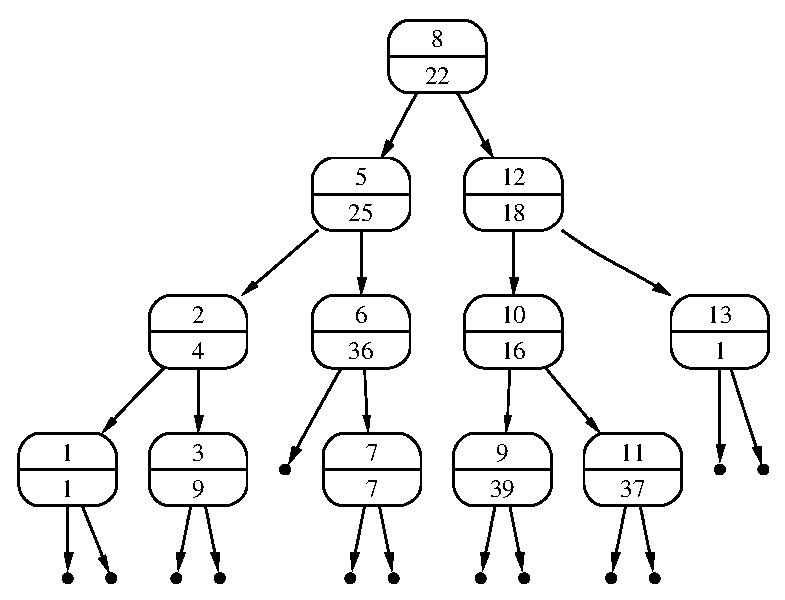
\epsfig{file=Abbildungen/graph2.eps}} 
  \caption{The ordered binary tree from Figure  
          \ref{fig:graph1} after deleting the node with label $\pair(4,16)$.}
  \label{fig:graph2}
\end{figure}

Next, we specify the  method \mytt{delMin}.  The signature is
\\[0.2cm]
\hspace*{1.3cm}
$\mytt{delMin}:\mathcal{B} \rightarrow \mathcal{B} \times \textsl{Key} \times \textsl{Value}$.
\\[0.2cm]
\index{\mytt{delMin}, ordered binary tree}
Hence, the call $t.\mytt{delMin}()$ returns a triple: If 
\\[0.2cm]
\hspace*{1.3cm}
$t.\mytt{delMin}() = \langle r,k,v \rangle$,
\\[0.2cm]
then $r$ is the tree that  results from
removing the smallest key in $t$, $k$ is the key that is removed and $v$ is the associated value.
\begin{enumerate}
\item $\mytt{Node}(k, v, \mytt{Nil}, r).\mytt{delMin}() = \langle r, k, v\rangle$

      If the left subtree is empty, $k$ has to be the smallest key in the tree 
      $\mytt{Node}(k, v, \mytt{Nil}, r)$.  If $k$ and its associated value $v$ are removed, we are left with the subtree $r$.
\item $l\not= \mytt{Nil} \wedge l.\mytt{delMin}() = \langle l',k_{min}, v_{min}\rangle \;\rightarrow$ \\[0.2cm]
       \hspace*{1.3cm} 
       $\mytt{Node}(k, v, l, r).\mytt{delMin}() = \bigl\langle\mytt{Node}(k, v, l', r), k_{min}, v_{min})\bigr\rangle$.

      If the left subtree $l$ in the binary tree $t = \mytt{Node}(k, v, l, r)$
      is not empty, then the smallest key of  $t$ is located inside the left subtree $l$.
      This smallest key is recursively removed from  $l$. This yields the tree 
      $l'$.  Next,  $l$ is replaced by $l'$ in $t$.  The resulting tree is
      $t' = \mytt{Node}(k, v, l', r)$.
\end{enumerate}
Finally, we specify the method $\mytt{delete}()$.
\begin{enumerate}
\item $\mytt{Nil}.\mytt{delete}(k) = \mytt{Nil}$.
\item $\mytt{Node}(k,v,\mytt{Nil},r).\mytt{delete}\bigl(k\bigr) = r$.
\item $\mytt{Node}(k,v,l,\mytt{Nil}).\mytt{delete}(k) = l$.
\item $l \not= \mytt{Nil} \,\wedge\, r \not= \mytt{Nil} \,\wedge\, \langle r',k_{min}, v_{min}\rangle := r.\mytt{delMin}() \;\rightarrow$ \\[0.2cm]
      \hspace*{1.3cm}
      $\mytt{Node}(k,v,l,r).\mytt{delete}(k) = \mytt{Node}(k_{min},v_{min},l,r')$.
      
      If the key $k$ to be removed is found at the root of the tree and neither of its subtrees is
      empty, the call  $r\mytt{.}\mytt{delMin}()$ removes the smallest key together with its
      associated value from the subtree $r$ yielding the subtree $r'$.
      The smallest key from $r$ is then stored at the root of the new tree.

\item $k_1 < k_2 \rightarrow \mytt{Node}(k_2,v_2,l,r).\mytt{delete}\bigl(k_1) = 
       \mytt{Node}(k_2,v_2,l.\mytt{delete}(k_1),r)$.

       If the key $k_1$ that is to be removed is less than the key $k_2$ stored at the root, the key $k_1$ can only be
       located in the left subtree $l$.  Hence, $k_1$ is removed from the left subtree $l$ recursively.
\item $k_1 > k_2 \rightarrow \mytt{Node}(k_2,v_2,l,r).\mytt{delete}(k_1) = 
       \mytt{Node}(k_2,v_2,l,r.\mytt{delete}(k_1))$.

       If the key $k_1$ that is to be removed is greater than the key stored at the root, the key $k_1$ can only be
       located in the right subtree $r$.  Hence, $k_1$ is removed from the right subtree $r$ recursively.
\end{enumerate}

\subsection{Implementing Ordered Binary Trees in \textsl{Python}}
Figure \ref{fig:binary-tree.py-1} and Figure \ref{fig:binary-tree.py-2} show how ordered binary
trees can be implemented in \textsl{Python}.  Objects of class \mytt{OrderedBinaryTree} represent ordered
binary trees.  We discuss the implementation of this class next.
\begin{enumerate}
\item The constructor is called without any argument.  The expression
      \\[0.2cm]
      \hspace*{1.3cm}
      $\mytt{OrderedBinaryTree()}$
      \\[0.2cm]
      creates an empty tree that corresponds to $\mytt{Nil}$.
\item The class \mytt{OrderedBinaryTree} represents a node in an ordered binary tree.  In order to do so, it
      maintains four additional member variables.
      \begin{enumerate}
      \item \mytt{mKey} is the key stored at this node.  For an empty node, \mytt{mKey}
            has the value \mytt{None}, which represents $\Omega$.
      \item \mytt{mValue} stores the value that is associated with \mytt{mKey}.  For an empty node,
            \mytt{mValue} is \mytt{None}.
      \item \mytt{mLeft} is the left subtree.  
      \item \mytt{mRight} is the right subtree.  
      \end{enumerate}
\item The function \mytt{isEmpty} checks whether \mytt{self} represents an empty tree.
      The assumption is that if \mytt{mKey} is \mytt{None}, then the member variables
      \mytt{mValue}, \mytt{mLeft}, and \mytt{mRight} will also be \mytt{None}.
      Hence, in this case the object represents the empty tree \mytt{Nil}.
\item The implementation of \mytt{find} works as follows:
      \begin{enumerate}
      \item If the node is empty, there is no value to find and the function returns \mytt{None}.
      \item If $\mytt{key} == \mytt{mKey}$, then the key we are looking for is stored at the root of this
            tree and hence the value we are looking for is \mytt{mValue}.
      \item Otherwise, we have to compare the key \mytt{key}, which is the key we are looking for,
            with the key \mytt{mKey}, which is the key stored in this node.  If \mytt{key}
            is less than \mytt{mKey}, the value associated with \mytt{key} can only be stored in the left subtree
            \mytt{mLeft}, while if \mytt{key} is greater than \mytt{mKey}, the value associated with
            \mytt{key} can only be stored in the right subtree \mytt{mRight}.
      \end{enumerate}


\begin{figure}[!ht]
  \centering
\begin{minted}[ frame         = lines, 
                framesep      = 0.3cm, 
                bgcolor       = sepia,
                numbers       = left,
                numbersep     = -0.2cm,
                xleftmargin   = 0.0cm,
                xrightmargin  = 0.0cm
              ]{python3}
    class OrderedBinaryTree:
        def __init__(self):
            self.mKey   = None
            self.mValue = None
            self.mLeft  = None
            self.mRight = None
    
        def isEmpty(self):
            return self.mKey == None
    
        def find(self, key):
            if self.isEmpty():
                return None
            elif self.mKey == key:
                return self.mValue
            elif key < self.mKey:
                return self.mLeft.find(key)
            else:
                return self.mRight.find(key)
    
        def insert(self, key, value):
            if self.isEmpty():
                self.mKey   = key
                self.mValue = value
                self.mLeft  = OrderedBinaryTree()
                self.mRight = OrderedBinaryTree()
            elif self.mKey == key:
                self.mValue = value
            elif key < self.mKey:
                self.mLeft.insert(key, value)
            else:
                self.mRight.insert(key, value)
\end{minted}
\vspace*{-0.3cm}
  \caption{Implementation of ordered binary trees in \textsl{Python}, part \mytt{I}.}
  \label{fig:binary-tree.py-1}
\end{figure}
\item The implementation of \mytt{insert} is similar to the implementation of \mytt{find}.
      \begin{enumerate}
      \item If the binary tree is empty, we set the member variables \mytt{mKey} and
            \mytt{mValue} to the appropriate values.  The member variables \mytt{mLeft} and 
            \mytt{mRight} are initialized as empty trees.
      \item If the key \mytt{key}, for which the value \mytt{value} is to be inserted, is identical
            to the key \mytt{mKey} stored at this node, then we have found the node where we need
            to insert \mytt{value}.  In this case, the current value of the variables \mytt{mValue} is
            overwritten with \mytt{value}. 
      \item Otherwise, \mytt{key} is compared with \mytt{mKey} and the insertion is recursively continued in the
            appropriate subtree.
      \end{enumerate}      


\begin{figure}[!ht]
  \centering
\begin{minted}[ frame         = lines, 
                framesep      = 0.3cm, 
                firstnumber   = last,
                bgcolor       = sepia,
                numbers       = left,
                numbersep     = -0.2cm,
                xleftmargin   = 0.8cm,
                xrightmargin  = 0.8cm
              ]{python3}
        def delete(self, key):
            if self.isEmpty():
                return
            if key == self.mKey:
                if self.mLeft.isEmpty():
                    self._update(self.mRight)
                elif self.mRight.isEmpty():
                    self._update(self.mLeft)
                else:
                    rs, km, vm = self.mRight._delMin()
                    self.mKey   = km
                    self.mValue = vm
                    self.mRight = rs
            elif key < self.mKey:
                self.mLeft.delete(key)
            else:
                self.mRight.delete(key)
    
        def _delMin(self):
            if self.mLeft.isEmpty():
                return self.mRight, self.mKey, self.mValue
            else:
                ls, km, vm = self.mLeft._delMin()
                self.mLeft = ls
                return self, km, vm

        def _update(self, t):
            self.mKey   = t.mKey
            self.mValue = t.mValue
            self.mLeft  = t.mLeft
            self.mRight = t.mRight
\end{minted}
\vspace*{-0.3cm}
  \caption{Implementation of ordered binary trees in \textsl{Python}, part \mytt{II}.}
  \label{fig:binary-tree.py-2}
\end{figure}

\item The implementation of \mytt{delMin} and \mytt{delete} is done in a similar way as the
      implementation of \mytt{insert}.  It should be noted that the implementation follows directly from the
      equations derived  previously. 
      
      There is however one caveat that should be mentioned.  Line 59 show the implementation of the
      function \mytt{update}.  When we delete the key at the root of the tree and either of the
      subtrees is empty, we would like to overwrite the current tree with the non-empty
      subtree, i.e.~we would like to write something like
      \\[0.2cm]
      \hspace*{1.3cm}
      \mytt{self = mLeft}
      \\[0.2cm]
      However, we cannot replace the object \mytt{self} with another object.  The only thing we can do is
      change the attributes of the object \mytt{self}.  This is done in the method \mytt{update}.
      The expression \mytt{self.update(t)} overwrites the member variables of the object \mytt{self} with the
      corresponding member variables of the ordered binary tree \mytt{t}. 
\end{enumerate}

\begin{figure}[!th]
  \centering 
  \framebox{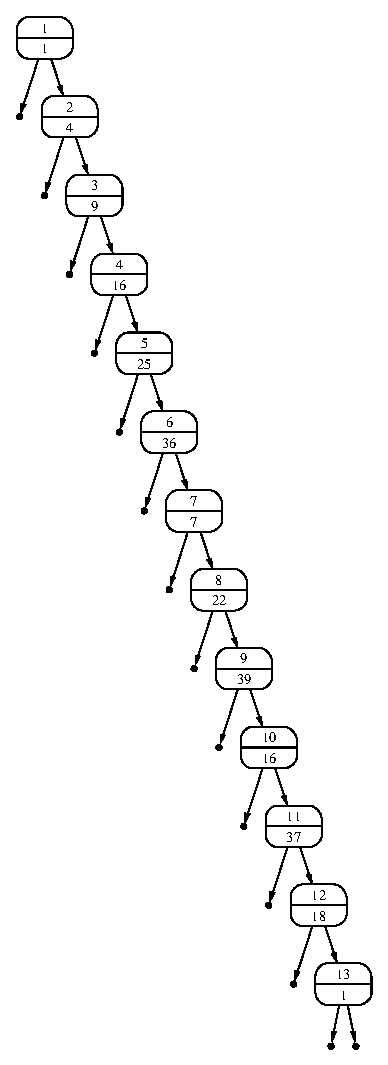
\epsfig{file=Abbildungen/degenerated-bin-tree}} 
  \caption{A degenerated binary tree.}
  \label{fig:degenerated}
\end{figure}


\subsection{Complexity Analysis}
In this section we will first discuss the \blue{worst case complexity} of ordered binary trees.  Unfortunately,
this complexity is quite bad.  In fact, in 
the worst case, the call $b.\mytt{find}(k)$ will perform $\Oh(n)$ key comparisons if $b$ is an ordered
binary search tree containing $n$ key-value pairs.  After that, we investigate the \blue{average case complexity}.  We
will show that the average case complexity is $\Oh\bigr(\ln(n)\bigr)$.

\subsubsection{Worst Case Complexity}
We begin our investigation of the complexity with an analysis of the complexity of $b.\mytt{find}(k)$ 
in the worst case.  The worst case happens if the binary tree $b$ degenerates into a list.
Figure \ref{fig:degenerated} on page \pageref{fig:degenerated} shows an ordered binary tree that
is generated by inserting the keys in increasing order.  If we then have to search for the
biggest key, we have to traverse the complete tree in order to find this key.  Therefore, if the
tree $b$ contains $n$ different keys, we have to compare the key $k$ that we are looking for to all
of these $n$ keys in the tree.  Hence, in this case the complexity of $b.\mytt{find}(k)$ is 
$\Oh(n)$ and this is the same complexity that we would have gotten if we had used a linked list.


\subsubsection{Average Case Complexity}
Fortunately, the worst case has a very small probability to occur if the keys are inserted randomly\footnote{
  In practice, keys are not generated randomly.  Therefore, in practice the worst case is not that unlikely to occur.
}. On average, a randomly generated
binary tree is quite well balanced.  We will show next that the number of comparisons necessary for
the function call $b.\mytt{find}(k)$ has the order $\Oh\bigl(\ln(n)\bigr)$.  


%Dazu definieren wir auf bin\"aren B\"aumen zun\"achst eine Funktion 
%\[ \mytt{height}: \Bin \rightarrow \N, \]
%die die H\"ohe eines bin\"aren Baums angibt.  Die Definition erfolgt induktiv.
%\begin{enumerate}
%\item $\mytt{Nil}.\mytt{height}() = 0$.

%      Der leere Baum hat die H\"ohe $0$.
%\item $\mytt{Node}(k,v,l,r).\mytt{height}() = 
%       1 + \max\bigl(l.\mytt{height}(),\, r.\mytt{height}()\bigr)$.

%      Die H\"ohe des Baums $\mytt{Node}(k,v,l,r)$ ist um eins gr\"o{\ss}er als die H\"ohe des
%      gr\"o{\ss}ten Teilbaums.
%\end{enumerate}
%Analog definieren wir f\"ur einen bin\"aren Baum $b$ die Anzahl $b.\mytt{count}()$ der Schl\"ussel, die
%der Baum enth\"alt.   Die Definition von $b.\mytt{count}()$ erfolgt durch Induktion nach $b$.
%\begin{enumerate}
%\item $\mytt{Nil}.\mytt{count}() = 0$.

%      Der leere Baum enth\"alt keine Schl\"ussel.
%\item $\mytt{Node}(k,v,l,r).\mytt{count}() = 
%       1 + l.\mytt{count}() + r.\mytt{height}()\bigr)$.

%      Der Baum $\mytt{Node}(k,v,l,r)$ enth\"alt zus\"atzlich zu dem Schl\"ussel $k$ die
%      Schl\"ussel aus den Teilb\"aumen $l$ und $r$.
%\end{enumerate}
%Der folgende Satz zeigt, wieviel Schl\"ussel ein Baum der H\"ohe $h$ h\"ochstens enthalten
%kann.

%\begin{Satz}
%  Ein bin\"arer Baum $b$ der H\"ohe $h$ enth\"alt h\"ochstens $2^h - 1$ Schl\"ussel.
%\end{Satz}
%\noindent
%\textbf{Beweis}:  Wir bezeichnen die maximale Anzahl Schl\"ussel eines Baums der H\"ohe $h$
%mit $c_h$.  Wir beweisen  durch Induktion nach $h$, dass gilt:
%\[ c_h = 2^h - 1. \]
%\begin{enumerate}
%\item[I.A.] $h = 0$: Der einzige Baum der H\"ohe $0$ ist $\mytt{Nil}$.
%            Dieser enth\"alt $0$ Schl\"ussel.  Also gilt
%            \\[0.2cm]
%            \hspace*{1.3cm}
%            $c_0 = 0 = 2^0 - 1$.
%\item[I.S.] $h \mapsto h + 1$: Ein Baum der H\"ohe $h+1$, der die maximale Anzahl
%            Schl\"ussel enth\"alt, hat die Form $\mytt{Node}(k,v,l,r)$, wobei dann $l$ und
%            $r$  B\"aume der H\"ohe $h$ sind, die die maximale Anzahl Schl\"ussel enthalten.
%            Folglich gilt:
%            \begin{eqnarray*}
%               c_{h+1} &               =  & 1 + c_h + c_h \\
%                       & \stackrel{IV}{=} & 1 + (2^h - 1) + (2^h - 1) \\
%                       &               =  & 2 \cdot 2^h - 1 \\
%                       &               =  & 2^{h+1} - 1. \hspace*{9cm} \Box
%            \end{eqnarray*}
%\end{enumerate}

%Die H\"ohe eines Baumes gibt ein Ma{\ss} f\"ur die Komplexit\"at der Methoden \mytt{find},
%\mytt{insert} und \mytt{delete}, denn bei einem Baum der H\"ohe $h$ sind f\"ur jede dieser
%Operationen h\"ochstens $h$ Vergleiche von Schl\"usseln erforderlich.

In order to prove this claim, we have to introduce some definitions.
We define the \underline{avera}g\underline{e} number of comparisons that are needed for the function
call $b.\mytt{find}(k)$ as  $d_n$, where $n$ is the number of keys stored in $b$.  We assume that
the key $k$ is indeed stored in $b$.  Our first goal is to derive a recurrence equation for 
$d_n$.  First, we note that  
\\[0.2cm]
\hspace*{1.3cm} $d_1 = 1$,
\\[0.2cm]
because if the tree $b$ contains only one key we need exactly one key comparison.
Next, imagine a binary tree $b$ that contains $n+1$ keys.  Then $b$
can be written as 
\\[0.2cm]
\hspace*{1.3cm}
$b = \mytt{Node}\bigl(\bar{k},v,l,r\bigr)$,
\\[0.2cm]
where $\bar{k}$ is the key at the root of $b$.  If the keys of $b$ are ordered as a list, then this
ordering looks something like the following:
\\[0.2cm]
\hspace*{1.3cm}
$k_0 < k_1 < \cdots < k_{i-1} < k_{i} < k_{i+1} < \cdots < k_{n-1} < k_n$.
\\[0.2cm]
Here, there are $n+1$ positions for the key $\bar{k}$.
If we have $\bar{k} = k_i$, then the left subtree of $b$ contains  $i$ keys while the right subtree
contains the remaining  $n-i$ keys:
\\[0.2cm]
\hspace*{1.3cm}
$\underbrace{k_0 < k_1 < \cdots < k_{i-1}}_{\mbox{keys in $l$}} < 
 \underbrace{k_{i}}_{\displaystyle \bar{k}} < 
 \underbrace{k_{i+1} < \cdots < k_{n-1} < k_n}_{\mbox{keys in $r$}}$,
\\[0.2cm]
As  $b$ contains $n+1$ keys all together, there are  $n+1$ different possibilities for the position
of $\bar{k}$, as the number of keys in the left subtree $l$ is $i$ where
\\[0.2cm]
\hspace*{1.3cm}
 $i \in \{0,1, \cdots, n\}$.
\\[0.2cm]
Of course, if the left subtree has $i$ keys, the right subtree will have $n-i$ keys.
Let us denote the average number of comparisons that are done during the function call
$b.\mytt{find}(k)$ provided the left subtree of $b$ has $i$ keys while $b$ itself has $n+1$ keys
as
\\[0.2cm]
\hspace*{1.3cm}
$\mytt{numCmp}(i,\, n\!+\!1)$.
\\[0.2cm]
Then, since all values of $i$ are assumed to have the same probability, we have
\\[0.2cm]
\hspace*{1.3cm}
$\ds d_{n+1} =  \frac{1}{n+1} \cdot \sum\limits_{i=0}^n \mytt{numCmp}(i,\, n\!+\!1)$.
\\[0.2cm]
We proceed to compute $\mytt{numCmp}(i,n\!+\!1)$:
If  $l$ contains $i$ keys while $r$ contains the remaining $n-i$ keys,
then there are three possibilities for the key $k$ that we want to find in $b$:
\begin{enumerate}
\item $k$ might be identical with the key $\bar{k}$ that is located at the root of $b$.
      In this case there is only one comparison.
      As there  are $n+1$ keys in $b$ and the key we are looking for will be at the root in only
      one of these cases, the probability of this case is
      \\[0.2cm]
      \hspace*{1.3cm} $\bruch{1}{\,n+1\,}$.

\item $k$ might be identical to one of the  $i$ keys of the left subtree $l$.
      The probability for this case is 
      \\[0.2cm]
      \hspace*{1.3cm} $\displaystyle\bruch{i}{n+1}$. \\[0.2cm]
      In this case we need 
      \\[0.2cm]
      \hspace*{1.3cm} $\displaystyle d_i + 1$ \\[0.2cm]
      comparisons because in addition to the  $d_i$ comparisons in the left subtree we have to
      compare the key $k$ we are looking for with the key $\bar{k}$ at the root of the tree.
\item $k$ might be a key in the right subtree $r$.  As there are  $n-i$ keys in the right subtree
      and the total of keys is $n+1$, the probability that the key  $k$ occurs in the right subtree $r$
      is \\[0.2cm]
      \hspace*{1.3cm} $\displaystyle \bruch{n-i}{n+1}$. \\[0.2cm]
      In this case there are  \\[0.2cm]
      \hspace*{1.3cm} $\displaystyle d_{n-i} + 1$ \\[0.2cm]
      comparisons. 
\end{enumerate}
In order to compute  $\mytt{numCmp}(i, n\!+\!1)$ we have to multiply the probabilities in every
case with the number of comparisons and these three numbers have to added.  This yields
\begin{eqnarray*}
  \mytt{numCmp}(i, n\!+\!1) 
& = & \bruch{1}{\,n+1\,} \cdot 1 + \bruch{i}{n+1} \cdot (d_i + 1) + \bruch{n-i}{n+1} \cdot (d_{n-i} + 1) 
      \\[0.2cm]
& = & \bruch{1}{\,n+1\,} \cdot \bigl(1 + i \cdot (d_i + 1) + (n-i) \cdot (d_{n-i} + 1)\bigr)      \\[0.2cm]
& = & \bruch{1}{\,n+1\,} \cdot \bigl(1 + i + (n-i) + i \cdot d_i + (n-i) \cdot d_{n-i} \bigr)    \\[0.2cm]
& = & \bruch{1}{\,n+1\,} \cdot \bigl(n + 1 + i \cdot d_i + (n-i) \cdot d_{n-i} \bigr)            \\[0.2cm]
& = & 1 + \bruch{1}{\,n+1\,} \cdot \bigl(i \cdot d_i + (n-i) \cdot d_{n-i} \bigr) 
\end{eqnarray*}


Therefore, the recurrence equation for $d_{n+1}$ is given as follows: 
\\[0.2cm]
\hspace*{1.3cm}
$
\begin{array}{lcl}
d_{n+1} 
& = &  
\ds\sum\limits_{i=0}^n \bruch{1}{\,n+1\,} \cdot \mytt{numCmp}(i,\,n\!+\!1)  \\[0.5cm]
& = &  
\ds\bruch{1}{n+1} \cdot \sum\limits_{i=0}^n  
           \left(1 + \bruch{1}{n+1} \cdot \bigl(i \cdot d_i + (n-i) \cdot d_{n-i} \bigr) \right)
\\[0.5cm]
& = &  
\bruch{1}{n+1} \cdot \Biggl(\underbrace{\sum\limits_{i=0}^n 1}_{n+1} \;+\;
           \bruch{1}{n+1} \cdot \ds\sum\limits_{i=0}^n \bigl(i \cdot d_i + (n-i) \cdot d_{n-i} \bigr) \Biggr)
\\[1.3cm]
& = &  
1 + \bruch{1}{(n+1)^2} \cdot \left(\ds\sum\limits_{i=0}^n \left(i\cdot d_i + (n-i)\cdot d_{n-i}\right) \right) 
\\[0.5cm]
& = &  
1 + \bruch{2}{(n+1)^2} \cdot \ds\sum\limits_{i=0}^n i\cdot d_i 
\end{array}
$
\\[0.2cm]
Here we have used the fact that the identity  \\[0.2cm]
\hspace*{1.3cm}
$\ds\sum\limits_{i=0}^n a_{n-i} = \sum\limits_{i=0}^n a_i$ \\[0.2cm]
is valid for any sequence $(a_n)_{n}$.
We had verified this equation already when discussing the complexity of \blue{QuickSort} in the average
case.  Next, we solve the recurrence equation 
\begin{equation}
  \label{eq:bin1}
d_{n+1} = \displaystyle 1 + \bruch{2}{(n+1)^2} \cdot \sum\limits_{i=0}^n i\cdot d_i  
\end{equation}
with the initial condition $d_1 = 1$.  
In order to solve the equation (\ref{eq:bin1}) we perform the substitution $n \mapsto n+1$.  This yields
\begin{equation}
  \label{eq:bin2}
d_{n+2} = \displaystyle 1 + \bruch{2}{(n+2)^2} \cdot \sum\limits_{i=0}^{n+1} i\cdot d_i  
\end{equation}
We multiply equation (\ref{eq:bin1}) with $(n+1)^2$ and equation (\ref{eq:bin2}) 
with $(n+2)^2$.  We get
\begin{eqnarray}
  \label{eq:bin3}
(n+1)^2 \cdot d_{n+1} & = & (n+1)^2 + 2 \cdot \sum\limits_{i=0}^n i\cdot d_i, \\
  \label{eq:bin4}
(n+2)^2 \cdot d_{n+2} & = & (n+2)^2 + 2 \cdot \sum\limits_{i=0}^{n+1} i\cdot d_i
\end{eqnarray}
We subtract equation  (\ref{eq:bin3}) from equation (\ref{eq:bin4})
and are left with \\[0.2cm]
\hspace*{1.3cm} 
$(n+2)^2 \cdot d_{n+2} - (n+1)^2 \cdot d_{n+1} = (n+2)^2 - (n+1)^2 + 2 \cdot (n+1) \cdot d_{n+1}$.
\\[0.2cm]
To simplify this equation we substitute  $n \mapsto n - 1$ and get \\[0.2cm]
\hspace*{1.3cm} 
$(n+1)^2 \cdot d_{n+1} - n^2 \cdot d_{n} = (n+1)^2 - n^2 + 2 \cdot n \cdot d_{n}$.
\\[0.2cm]
This can be simplified as \\[0.2cm]
\hspace*{1.3cm} $(n+1)^2 \cdot d_{n+1}  =  n \cdot (n + 2) \cdot d_{n} + 2 \cdot n + 1$. \\[0.2cm]
Let us divide both sides of this equation by $(n+2)\cdot (n+1)$.  We get \\[0.2cm]
\hspace*{1.3cm}  
$\displaystyle \bruch{n+1}{n+2} \cdot d_{n+1}  =  \bruch{n}{n + 1} \cdot d_{n} + \bruch{2 \cdot n + 1}{(n+2)\cdot (n+1)}$. \\[0.2cm]
We define \\[0.2cm]
\hspace*{1.3cm} $\displaystyle c_n = \bruch{n}{n+1} \cdot d_n$. \\[0.4cm]
Then $c_1 = \bruch{1}{2} \cdot d_1 = \bruch{1}{2}$ and hence we have found the recurrence equation \\[0.2cm]
\hspace*{1.3cm} 
$\displaystyle c_{n+1}  =  c_{n} + \frac{2 \cdot n + 1}{(n+2)\cdot (n+1)}$ \quad with the initial condition $\ds c_1 = \frac{1}{2}$.
\\[0.2cm]
A partial fraction decomposition shows that \\[0.2cm]
\hspace*{1.3cm} 
$\displaystyle \frac{2 \cdot n + 1}{(n+2)\cdot (n+1)} = \frac{3}{n+2} - \frac{1}{n+1}$. \\[0.2cm]
Hence we have \\[0.2cm]
\hspace*{1.3cm} $\displaystyle c_{n+1} = c_n +  \frac{3}{n+2} - \frac{1}{n+1}$. \\[0.2cm]
Because of $c_1 = \bruch{1}{2}$ this equation is also valid for  $n=0$ if we define $c_0 := 0$, since
we have
\\[0.2cm]
\hspace*{1.3cm}
$\bruch{1}{2} = 0 + \bruch{3}{0+2} - \bruch{1}{0+1}$.
\\[0.2cm]
The recurrence equation for $c_n$ can be solved using  \blue{telescoping}:
\begin{eqnarray*}  
  c_{n+1} & = & c_0 + \sum\limits_{i=0}^{n} \frac{3}{i+2} - \sum\limits_{i=0}^{n} \frac{1}{i+1} 
\\[0.2cm]
          & = & \sum\limits_{i=2}^{n+2} \frac{3}{i} - \sum\limits_{i=1}^{n+1} \frac{1}{i}.
\end{eqnarray*}
To simplify this equation we substitute $n \mapsto n-1$ and get
\\[0.2cm]
\hspace*{1.3cm}
$c_{n} =  \displaystyle\sum\limits_{i=2}^{n+1} \frac{3}{i} - \sum\limits_{i=1}^{n} \frac{1}{i}$
\\[0.2cm]
The harmonic number  $H_n$ is defined as 
$H_n = \ds\sum\limits_{i=1}^{n} \bruch{1}{i}$.   
Therefore,  $c_n$ can be reduced to $H_n$: 
\\[0.2cm]
\hspace*{1.3cm}
$c_n = \ds 3 \cdot H_n - \frac{3}{1} + \frac{3}{n+1} - H_n  =  \ds 2 \cdot H_n - 3 \cdot \frac{n}{n+1}$
\\[0.2cm] 
Because $H_n = \displaystyle\sum\limits_{i=1}^{n} \frac{1}{i} = \ln(n) + \Oh(1)$ and $\ds 3 \cdot\frac{n}{n+1} \in \Oh(1)$
we therefore have shown that
  \\[0.3cm]
\hspace*{1.3cm} 
$\displaystyle c_n = 2 \cdot \ln(n) + \Oh(1)$.
\\[0.3cm]
Because of  $d_n = \frac{n+1}{n}\cdot c_n$ this implies \\[0.2cm]
\hspace*{1.3cm}
 $\displaystyle d_n = 2 \cdot \ln(n) + \Oh\bigl(1\bigr)$.
\\[0.2cm]
This is our main result:  On average, the operation $b.\mytt{find}(k)$ uses
\\[0.2cm]
\hspace*{1.3cm}
$2 \cdot \ln(n) = 2 \cdot \ln(2) \cdot \log_2(n) \approx 1.386 \cdot \log_2(n)$ 
\\[0.2cm]
comparisons.  Hence in the average case there are about  39 \% 
more comparisons than there would be if the tree was optimally balanced.
There are similar results for the operations \mytt{insert} and \mytt{delete}.

\exercise
Use ordered binary trees to implement a function \mytt{treeSort} that takes a list of numbers \mytt{L} as
its input and returns a sorted list \mytt{S} that contains every element of  \mytt{L} exactly once.  If
$n$ is the length of \mytt{L}, the average complexity of your implementation should be $\Oh\bigl(n \cdot \log_2(n)\bigr)$. \eox


%%% Local Variables: 
%%% mode: latex
%%% TeX-master: "algorithms"
%%% End: 
